% Numbers: figures/results_summary.json and figures/results_annual.csv (built by figures/make_results.py).
\section{Results}
\label{sec:results}

\subsection{Portfolio Performance}
\label{sec:performance-results}

Over 2016--2025 the strategy compounded at 15.95\% after tax against 14.21\% for the No-TLH account, ending with \$4.39 million versus \$3.77 million (Table~\ref{tab:summary}). The gap splits into about 1\% of higher pre-tax return and 0.75\% of tax alpha, defined as the reduction in tax drag against No-TLH, which tracks SPY monthly under the same costs and tax rules:
\begin{equation}
  \alpha_{\mathrm{tax}}=\big(R^{\mathrm{after}}_{\mathrm{Strategy}}-R^{\mathrm{pre}}_{\mathrm{Strategy}}\big)-\big(R^{\mathrm{after}}_{\mathrm{No\text{-}TLH}}-R^{\mathrm{pre}}_{\mathrm{No\text{-}TLH}}\big),
  \label{eq:taxalpha}
\end{equation}
with $R$ the compound annual growth rate.

\begin{table}[!h]
\caption{Full-period results, January 2016 -- December 2025}
\label{tab:summary}
\small
\begin{tabularx}{\linewidth}{@{}Lrrr@{}}
\toprule
 & \textsf{\textbf{Strategy}} & \textsf{\textbf{No-TLH}} & \textsf{\textbf{S\&P 500 TR}} \\
\midrule
Pre-tax CAGR & 15.76\% & 14.77\% & 15.01\% \\
After-tax CAGR & 15.95\% & 14.21\% & -- \\
After-tax Wealth & \$4.39M & \$3.77M & -- \\
Tax Alpha & 0.75\% & -- & -- \\
Recognized Losses, Short-Term & \$336{,}434 & \$8{,}628 & -- \\
Recognized Losses, Long-Term & \$59{,}923 & \$52{,}978 & -- \\
Pre-tax Alpha vs.\ S\&P 500 TR & $+$0.75\% & $-$0.24\% & -- \\
Realized Tracking Error & 1.24\% & 0.50\% & -- \\
Average Ex-ante Tracking Error & 1.00\% & -- & -- \\
Maximum Drawdown & $-$33.7\% & $-$33.1\% & $-$33.8\% \\
Average Annual Turnover & 42.3\% & 3.9\% & -- \\
Trading Costs & \$7{,}133 & \$1{,}198 & -- \\
Average Holdings & 411 & 503 & -- \\
\bottomrule
\end{tabularx}
\end{table}

\begin{figure}[!h]
\centering
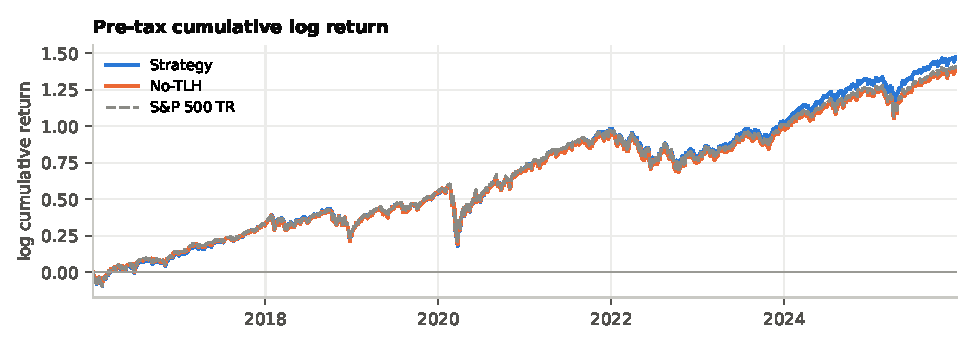
\includegraphics[width=\linewidth]{figures/fig_performance.pdf}
\caption{Pre-tax cumulative log return.}
\label{fig:performance}
\end{figure}

The strategy beat the S\&P 500 TR by 0.75\% a year (Figure~\ref{fig:performance}), but the gap is concentrated in 2024, when the strategy outperformed by 4.8\%. Excluding 2024, the annual gap is 0.34\%. The optimizer forecasts no returns, so this gap reflects active risk rather than a repeatable source of return. Drawdowns were in line with the index. The No-TLH account trailed the index by 0.24\% a year, mainly because about 2\% of its value sat in uninvested cash after whole-share rounding.

\begin{figure}[!h]
\centering
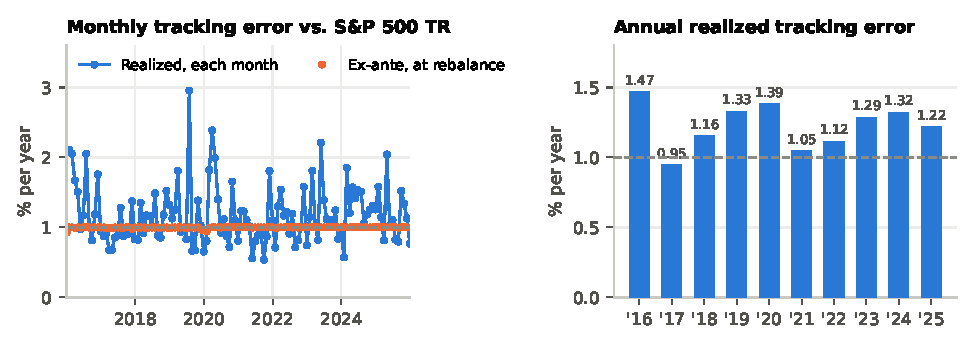
\includegraphics[width=\linewidth]{figures/fig_tracking.pdf}
\caption{Left: realized tracking error within each month (annualized from daily returns) and ex-ante tracking error at each rebalance. Right: realized tracking error by calendar year. Dashed lines mark the 1\% ex-ante limit.}
\label{fig:tracking}
\end{figure}

Ex-ante TE sat at the 1\% limit at almost every rebalance, while realized TE was 1.24\% over the full period. Month by month, realized TE had a median of 1.11\% and exceeded 1\% in 61\% of months (Figure~\ref{fig:tracking}). By calendar year, realized TE ranged from 0.95\% in 2017, the only year below the limit, to 1.47\% in 2016, when heavy harvesting moved the portfolio furthest from the index. The gap reflects drift between monthly rebalances, whole-share rounding and covariance estimation error. Targeting 1\% realized TE would require a tighter ex-ante limit.

\begin{figure}[!h]
\centering
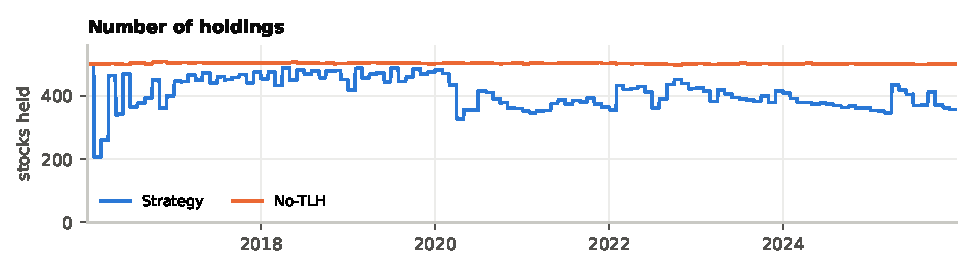
\includegraphics[width=\linewidth]{figures/fig_holdings.pdf}
\caption{Number of stocks held.}
\label{fig:holdings}
\end{figure}

Holdings fell from 502 to 207 in early 2016 as loss positions were sold and only partly replaced, then ranged between 330 and 480, ending at 357 against 501 for No-TLH (Figure~\ref{fig:holdings}). Average annual turnover of 42.3\% (Table~\ref{tab:summary}) is driven up by the first year: in 2016 the new portfolio harvested heavily and one-way turnover reached 183\%. Excluding 2016, turnover averaged 26.7\% a year (Table~\ref{tab:annual}). Of the \$2{,}332 spent on trading in 2016, only \$482 was the initial purchase. Most of the rest came from the February and March rebalances, when the strategy harvested the early-2016 losses.

\begin{table}[!h]
\caption{Annual results. Pre-tax alpha is against the S\&P 500 TR, and tax alpha is against No-TLH, both using calendar-year returns. Turnover is one-way, excluding the initial purchase. Trading cost includes the initial purchase.}
\label{tab:annual}
\small
\begin{tabularx}{\linewidth}{@{}Xrrrrrrrr@{}}
\toprule
\textsf{\textbf{Year}} & \textsf{\textbf{Strategy}} & \textsf{\textbf{S\&P 500 TR}} & \textsf{\textbf{Pre-tax $\alpha$}} & \textsf{\textbf{Tax $\alpha$}} & \textsf{\textbf{Realized TE}} & \textsf{\textbf{Turnover}} & \textsf{\textbf{Trading Cost}} & \textsf{\textbf{Holdings}} \\
\midrule
2016 & 12.1\% & 13.7\% & $-$1.55\% & $+$3.64\% & 1.47\% & 183\% & \$2{,}332 & 400 \\
2017 & 22.8\% & 21.8\% & $+$0.99\% & $+$0.50\% & 0.95\% & 48\% & \$600 & 476 \\
2018 & $-$4.4\% & $-$4.4\% & $-$0.05\% & $+$0.77\% & 1.16\% & 32\% & \$467 & 452 \\
2019 & 30.5\% & 31.5\% & $-$1.00\% & $+$0.85\% & 1.33\% & 30\% & \$454 & 476 \\
2020 & 18.9\% & 18.4\% & $+$0.52\% & $+$1.07\% & 1.39\% & 37\% & \$598 & 361 \\
2021 & 30.0\% & 28.7\% & $+$1.30\% & $-$0.13\% & 1.05\% & 12\% & \$285 & 365 \\
2022 & $-$17.2\% & $-$18.1\% & $+$0.92\% & $+$0.39\% & 1.12\% & 19\% & \$444 & 424 \\
2023 & 27.7\% & 26.3\% & $+$1.40\% & $+$0.55\% & 1.29\% & 29\% & \$734 & 417 \\
2024 & 29.8\% & 25.0\% & $+$4.77\% & $-$0.49\% & 1.32\% & 13\% & \$448 & 363 \\
2025 & 18.4\% & 17.9\% & $+$0.49\% & $+$0.10\% & 1.22\% & 20\% & \$771 & 357 \\
\bottomrule
\end{tabularx}
\end{table}

\subsection{Portfolio Aging}
\label{sec:aging}

Harvesting opportunities shrank as the portfolio aged. Recognized losses equaled 9.1\% of starting NAV in 2016, when every lot had just been bought near cost, and 1.8--3.8\% a year in 2017--2020 (Figure~\ref{fig:aging}). From 2021 they fell to 0.4--1.2\% in most years, with 2023 the exception at 2.8\%. Short-term losses made up 85\% of the \$396{,}000 recognized in total, since lots are most often below cost soon after purchase.

The cost basis fell from 97\% of NAV at inception to 29\% at the end of 2025, while unrealized gains rose to 71\% of NAV (Figure~\ref{fig:basis}). With no external cash flows, new lots come only from reinvested dividends, tax refunds and rebalancing trades, so most of the portfolio sits on gains that rising markets keep widening. Unrealized losses, the stock available to harvest, averaged 1.2\% of NAV in 2016 and only 0.3\% afterwards, rising briefly to 3.4\% in March 2020 and 1.4\% in 2022.

\begin{figure}[!h]
\centering
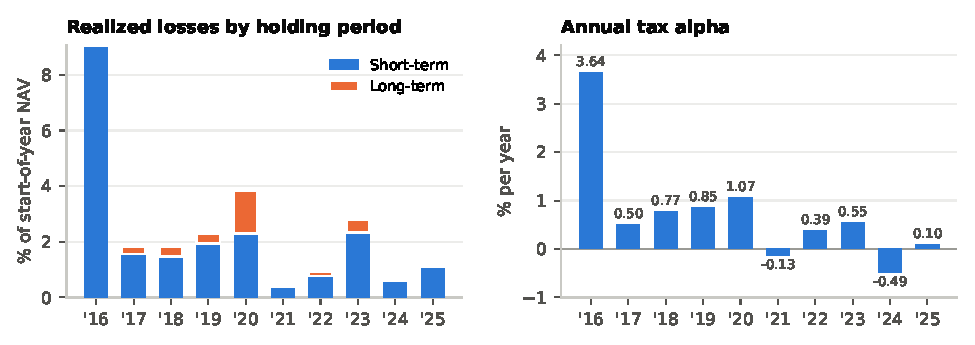
\includegraphics[width=\linewidth]{figures/fig_aging.pdf}
\caption{Left: recognized losses by holding period, as a share of NAV at the start of each year. Right: annual tax alpha against No-TLH.}
\label{fig:aging}
\end{figure}

\begin{figure}[!h]
\centering
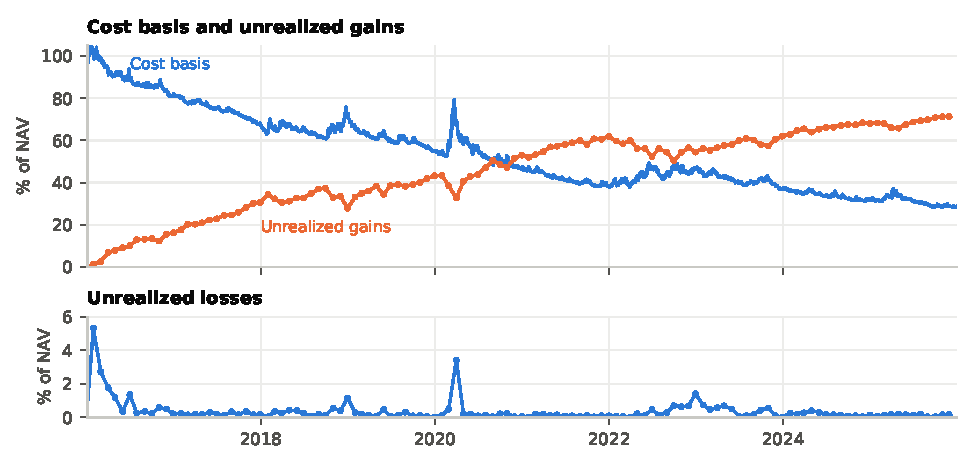
\includegraphics[width=\linewidth]{figures/fig_basis.pdf}
\caption{Top: aggregate cost basis (daily) and unrealized gains summed across lots (at each rebalance), as a share of NAV. Bottom: unrealized losses summed across lots, on their own scale.}
\label{fig:basis}
\end{figure}

Annual tax alpha followed the same path, from 3.64\% in 2016 to an average of 0.40\% in 2017--2025 (Figure~\ref{fig:aging}, right). Market conditions still matter. The 2016 peak partly reflects timing: the portfolio was bought on January 4, the first day of a global sell-off driven by China's stock market crash and oil falling below \$30 a barrel, and the S\&P 500 TR was down 8.9\% by February 11. The COVID-19 crash in March 2020 produced the largest losses after 2016, 3.8\% of NAV. The drawdown was deep enough to push even long-held lots below cost, so long-term losses reached 1.5\% of NAV, 40\% of that year's total and 45\% of all long-term losses over the decade. By contrast, the 2022 bear market produced only 0.9\% of NAV because most lots had appreciated well above cost by then. Strong markets work the other way. In 2021 and 2024 the S\&P 500 TR returned 28.7\% and 25.0\%, yet tax alpha was negative, at $-$0.13\% and $-$0.49\%. Few lots were below cost, so recognized losses fell to 0.4\% and 0.7\% of NAV, while rising prices pushed holdings away from benchmark weights. Trimming them back within the tracking-error limit realized gains, and the strategy paid more tax than No-TLH.

These patterns are consistent with portfolio lock-in. As embedded gains grow, correcting drift from the benchmark increasingly requires realizing gains, which can turn tax alpha negative. The backtest does not isolate this effect from market conditions, so lock-in remains a likely explanation rather than a demonstrated one.

\subsection{The Impact of the Wash-Sale Rule}
\label{sec:wash}
% Source: outputs/wash_metrics_20261122/wash_a (metrics.json, cohorts.json, annual.csv), traced from the final run's ledger.

The wash-sale rule deferred 19\% of harvested losses, but almost all of the deferral was brief. Over the decade the ledger recorded 2{,}593 wash-sale matches, which deferred \$92{,}895 of the \$489{,}252 in gross realized losses (Table~\ref{tab:wash}). Matches fell from 350--540 a year in 2016--2020 to fewer than 110 a year afterwards, in line with the smaller supply of losses in Figure~\ref{fig:aging}.

\begin{table}[!h]
\caption{Wash sales by year of the loss sale. A match pairs a loss sale with one replacement lot bought within 30 days. Gross loss splits into short-term (ST) and long-term (LT) losses. Still deferred is the part of that year's deferred losses not yet released at the end of 2025.}
\label{tab:wash}
\small
\begin{tabular*}{\linewidth}{@{\extracolsep{\fill}}lrrrrrrr@{}}
\toprule
\textsf{\textbf{Year}} & \textsf{\textbf{Matches}} & \textsf{\textbf{Gross Loss}} & \textsf{\textbf{ST Loss}} & \textsf{\textbf{LT Loss}} & \textsf{\textbf{Deferred}} & \textsf{\textbf{Deferred Share}} & \textsf{\textbf{Still Deferred}} \\
\midrule
2016 & 424 & \$118{,}446 & \$118{,}446 & \$0 & \$27{,}893 & 23.5\% & \$1{,}034 \\
2017 & 527 & \$24{,}543 & \$21{,}180 & \$3{,}362 & \$4{,}031 & 16.4\% & \$59 \\
2018 & 496 & \$32{,}294 & \$26{,}595 & \$5{,}699 & \$6{,}412 & 19.9\% & \$87 \\
2019 & 538 & \$36{,}617 & \$30{,}677 & \$5{,}940 & \$5{,}468 & 14.9\% & \$17 \\
2020 & 351 & \$77{,}497 & \$48{,}127 & \$29{,}369 & \$9{,}974 & 12.9\% & \$228 \\
2021 & 30 & \$9{,}418 & \$8{,}684 & \$733 & \$509 & 5.4\% & \$0 \\
2022 & 48 & \$29{,}114 & \$23{,}285 & \$5{,}830 & \$3{,}510 & 12.1\% & \$971 \\
2023 & 104 & \$79{,}824 & \$67{,}293 & \$12{,}531 & \$17{,}011 & 21.3\% & \$617 \\
2024 & 17 & \$26{,}647 & \$23{,}080 & \$3{,}568 & \$6{,}330 & 23.8\% & \$322 \\
2025 & 58 & \$54{,}853 & \$51{,}843 & \$3{,}010 & \$11{,}756 & 21.4\% & \$2{,}137 \\
\midrule
Total & 2{,}593 & \$489{,}252 & \$419{,}210 & \$70{,}042 & \$92{,}895 & 19.0\% & \$5{,}471 \\
\bottomrule
\end{tabular*}
\end{table}

The deferred share stayed between 12\% and 24\% in every year except 2021. By the end of 2025, \$87{,}424 of the \$92{,}895 deferred, or 94\%, had been released, after a median of 60 days, and 84\% were released within the same tax year, leaving that year's tax unchanged. Only \$5{,}471 remained deferred, worth about \$2{,}000 in tax. The largest share comes from 2025, whose replacement lots have had little time to be sold.

The rule therefore costs time value rather than tax savings. It delayed \$36{,}181 of tax benefit in total. Discounting each delayed benefit at 3--8\% a year gives a present-value cost of \$347--\$826 over ten years. Avoiding the rule outright is far more expensive. In a full-sample test that cancelled every wash-triggering order, wash sales disappeared, but after-tax CAGR fell by 1.34\% through cash drag, with cash peaking at 29.7\% of NAV, and drift from the benchmark.
